\documentclass{article}
\usepackage[a4paper, left=1.5cm, right=1.5cm, top=1cm, bottom=2cm]{geometry}

\usepackage{forest}
\usepackage{boldline}
\usepackage{tikz,tcolorbox}
\usepackage{amsmath}
\usepackage[table,xcdraw]{xcolor}
\usepackage{listings}
\usepackage{array,multirow} % For customizing tables
\usepackage{booktabs} % For better horizontal lines
\usepackage{makecell}
\setlength{\parindent}{0pt}
\usepackage{siunitx}
\usepackage{tkz-tab}
\usepackage{amssymb}
\usepackage{amsmath}
\usepackage{enumitem}

\usepackage{caption}
\usepackage{float}

\DeclareMathOperator*{\JoinOp}{\bowtie}


\newcommand{\exer}[1]{
  \section*{Exercice #1}
  \vspace{-0.5cm}
  \noindent\rule{\textwidth}{0.5pt}%
}

\newcommand{\tit}[1]{
\begin{center}
    \Large{\textbf{{#1}}}
\end{center}
}

\definecolor{commentgray}{HTML}{676160}
\definecolor{messagegreen}{HTML}{17B867}
\definecolor{myblue}{HTML}{10C2C4}

\newcounter{commentCount}
\newcounter{filePrg}
\newcounter{inputPrg}

\usepackage[dvipsnames]{xcolor}
\usepackage{minted}

\usepackage[many]{tcolorbox}
\tcbuselibrary{listings}
\tcbuselibrary{minted}

\usepackage{ifthen}
\usepackage{fontawesome}

\usepackage{tabularx}
\newcolumntype{\CeX}{>{\centering\let\newline\\\arraybackslash}X}%
\newcommand{\TwoSymbolsAndText}[3]{%
  \begin{tabularx}{\textwidth}{c\CeX c}%
    #1 & #2 & #3
  \end{tabularx}%
}

\newtcblisting[use counter=inputPrg, number format=\arabic]{codeInput}[4]{
  listing engine=minted,
  minted language=#1,
  minted options={autogobble,breaklines,  firstnumber={#4}},
  listing only,
  size=title,
  arc=1.5mm,
  breakable,
  enhanced jigsaw,
  colframe=myblue,
  coltitle=White,
  boxrule=0.5mm,
  colback=white,
  coltext=Black,
  title=\TwoSymbolsAndText{\faCode}{%
  \textbf{#2}%
  }{\faCode},
  label=inputPrg:#3
}




\tcbuselibrary{skins, breakable, theorems}
\usepackage{booktabs} 

\newtcolorbox{prettyBox}[2]{
  enhanced,
  colback=white!90!#2,   % Background color based on the second parameter (color)
  colframe=#2!60!black,  % Frame color based on the second parameter (color)
  coltitle=white,        % Title color (white)
  fonttitle=\bfseries\Large,
  title=#1,              % Title from the first parameter
  boxrule=1mm,
  arc=0.5mm,
  drop shadow=#2!35!gray, % Drop shadow color based on the second parameter (color)
}



\lstdefinestyle{cmd}{
 basicstyle=\ttfamily,
 backgroundcolor=\color{lightgray!20},
 frame=single
}

\lstdefinestyle{pythonstyle}{
    language=python,                    % Language set to Python
    basicstyle=\ttfamily\footnotesize,   % Change basic font size
    keywordstyle=\color{blue}\bfseries, % Different keyword style
    stringstyle=\color{red},         % Different string color
    commentstyle=\color{green!60!black}\itshape, % Adjust comment color
    numbers=left,                       % Line numbers on the left
    numberstyle=\tiny\color{gray},      % Smaller number font and color
    stepnumber=1,                       % Number each line
    frame=single,                       % Single frame around code
    tabsize=4,                          % Adjust tab size
    showstringspaces=false,             % Do not show spaces in strings
    captionpos=b,% Position of caption
    breaklines=true,
    inputencoding=utf8
}




\begin{document}
\tit{TD N\(^{\boldsymbol{\circ}}\)\hspace{0.1cm}4}

\vspace{0.35cm}


\begin{prettyBox}{Fragmentation}{myblue}
    La fragmentation permet de diviser une table en plusieurs sous-tables telles que
    la reconstruction de la table originale est toujours possible. Il y a deux types de
    fragmentation : \textbf{horizontale} et \textbf{verticale}.
\end{prettyBox}

\vspace{0.45cm}
\begin{prettyBox}{Fragmentation Horizontale}{myblue}
    On a deux types de fragmentation horizontale :
    \begin{itemize}
        \item \textbf{FHP (Fragmentation Horizontale Principale)} : on divise la table en utilisant l'opérateur de\\restriction $\sigma$ :
            \[
                \sigma_{\text{condition}} (\text{Table})
            \]
        \item \textbf{FHD (Fragmentation Horizontale Dérivée)} : on divise la table en utilisant l'opérateur de \\semi-jointure $\ltimes$ entre
            la table qui possède une clé étrangère faisant référence à une \textbf{FHP} :
            \[
                \text{Table} \ltimes \text{FHP}_{\text{référence}}
                = \text{Table} \bowtie \left( {\textstyle\prod_{\text{clé\_primaire}}} (\text{FHP}) \right)
            \]
    \end{itemize}

    L'opérateur de reconstruction est l'union $\bigcup$ :
    \[
        \text{Table} = \bigcup_{i=1}^{n} \text{Frag}_i
    \]
\end{prettyBox}

\vspace{0.45cm}
\begin{codeInput}{sql}{Fragmentation Horizontal}{code01}{41}
-- FHP
CREATE TABLE TABLE_NAME (
    ...
 )
 PARTITION BY LIST (ATTRIBUTE_NAME) (
    PARTITION FRAG1_NAME VALUES (VALUES_1),
    PARTITION FRAG2_NAME VALUES (VALUES_2),
    ....
    PARTITON FRAGN_NAME VALUES(DEFAULT) -- optional to use default means rest of values
 );

-- FHD
CREATE TABLE TABLE_NAME (
    ...,
CONSTRAINT CONSTRAINT_NAME foreign key(TABLE_NAME_FK) REFERENCES 
REFERENCED_TABLE(REFERENCES_TABLE_PK) ) PARTITION BY REFERENCE (CONSTRAINT_NAME);

\end{codeInput}

\newpage

\begin{prettyBox}{Fragmentation Verticale}{myblue}
    On utilise l'opérateur de projection $\prod$ :
    \[
        {\textstyle \prod_{\text{attribut}_1 , \dots , \text{attribut}_m}} (\text{Table})
    \]
    \textcolor{red}{\textbf{\large{Attention :}}} il faut toujours inclure la clé primaire dans les attributs de la projection afin de pouvoir
    faire la reconstruction avec l'opérateur de jointure $\bowtie$ :
    \[
        \text{Table} =  \JoinOp_{i=1}^{n}  \text{Frag}_i
    \]
\end{prettyBox}

\vspace{0.45cm}

\begin{codeInput}{sql}{Fragmentation Vertical}{code01}{41}
CREATE TABLE FRAG_NAME AS 
SELECT ATT_1 , ... , ATT_M FROM TABLE_NAME;
\end{codeInput}

\vspace{1cm}

\begin{prettyBox}{Arbre Algebrique}{myblue}
    \begin{enumerate}
        \item \textbf{Arbre Algebrique Global} :On utilise les tables d'origins.  
        \item \textbf{Arbre Algebrique Canonique} :on fait que remplacer les table avec leur fragments et
            utiliser l'operateur de reconstruction $\bigcup$ si horizontal , sinon si vertical $\JoinOp$
        \item \textbf{Arbre Simplifie} :
            \begin{itemize}
                \item \textbf{Regle d'optimisation Global} :descent des operateurs de reduction de taille\\ 
                    (projection,restriction) avant les operateurs $\bigcup$ et $\JoinOp$
                \item \textbf{Distribution Du Join Par Rapport A L'union} : 
                    \[A \JoinOp (B \bigcup C) = (A\JoinOp B) \bigcup (A \JoinOp C) \]
                \item \textbf{Supression Des Restrictions, Projection Inutiles}.
                \item \textbf{Supression Des Fragments Vides}.
            \end{itemize}
    \end{enumerate}
\end{prettyBox}

\newpage

\begin{prettyBox}{Schéma d'allocation}{myblue}
    Un schéma qui définit tout les sites avec leur fragments et tables de la base de données distribuée : 
\end{prettyBox}

\vspace{0.15cm}


\begin{figure}[H] 
  \centering 
  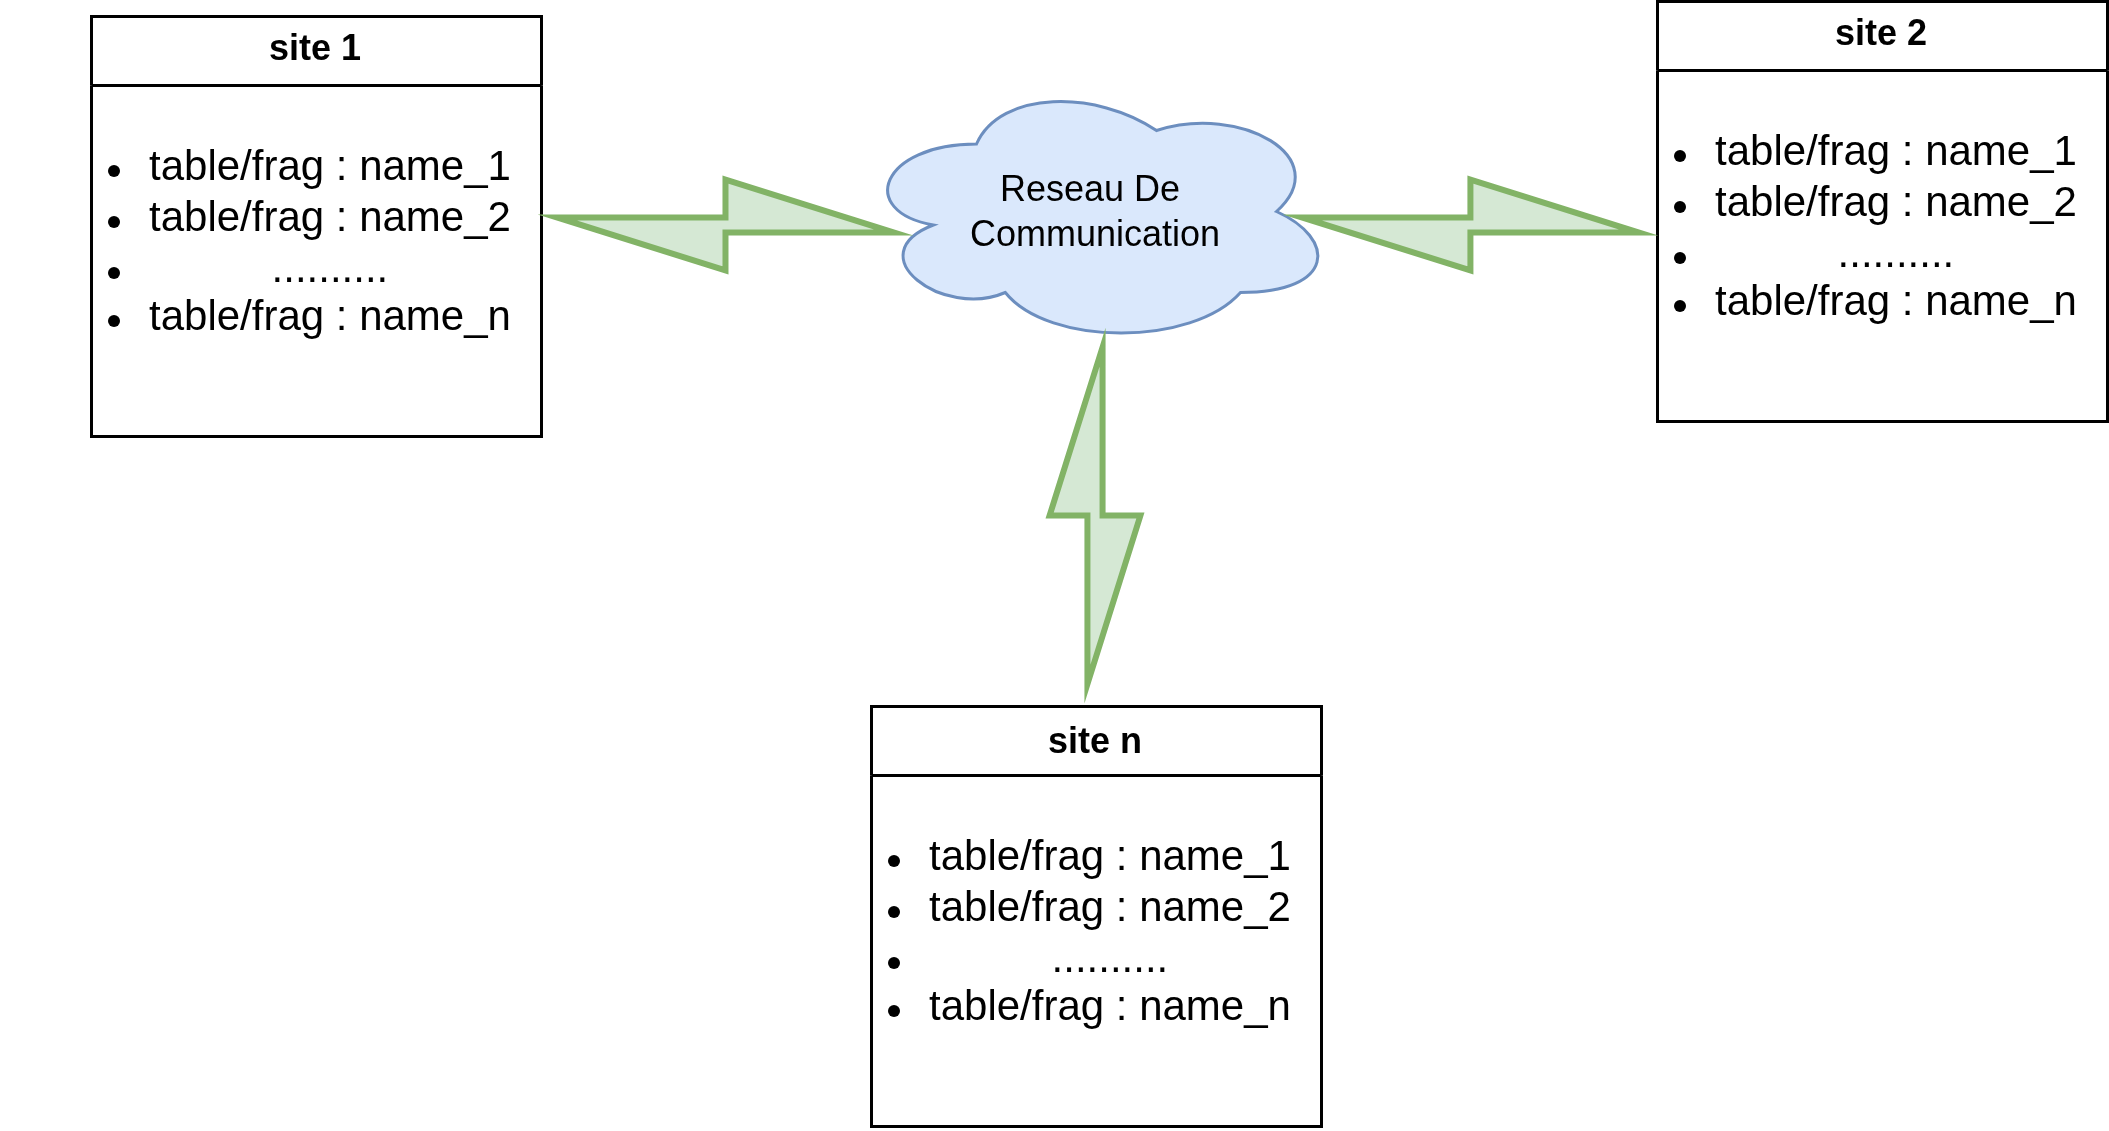
\includegraphics[width=0.65\textwidth]{alloc.png} 
\end{figure}

\vspace{0.5cm}

\begin{prettyBox}{Stratégie}{myblue}
    On a 3 cas global :
    \begin{itemize}
        \setlength{\itemsep}{0pt}
        \item Envoie tout les fragments/tables vers d'autre site et traiter la requete.
        \item Envoie les fragments/tables apres restriction/projection/jointure.
        \item Envoie des tuples de tout le fragments/table vers d'autre site qui ensuite vont repondre avec 
            un bit.
        \item Envoie des tuples de tout le fragments/table apres restriction/projection/jointure vers d'autre
            site qui ensuite vont repondre avec un bit.
    \end{itemize}
\end{prettyBox}

\vspace{0.5cm}
\begin{prettyBox}{Temps}{myblue}
    \[   \text{temp}_{envoie-table} = \text{delai-access} + \dfrac{\text{nb}_{\text{tuple}} \cdot \text{taille}_\text{tuple}}{\text{taux de transmission}}  \]
    
    \vspace{0.15cm}

    \[   \text{temp}_{envoie-bit} = \text{delai-access} + \dfrac{\text{taille}_\text{bit} = \frac{1}{8}}{\text{taux de transmission}}  \]
\end{prettyBox}

\newpage
\exer{1}

\vspace{0.25cm}

Fragmentation de production :\\[0.1cm]
Puisque l’entreprise a quatre sites et que chaque site est responsable de la production de différents composants, 
on va effectuer une fragmentation horizontale principale sur l’attribut composant.

\begin{alignat*}{2}
    &\text{Production}_{\text{UC}} &&= \sigma_{\text{Composant = 'Unite Centrale'}} (\text{Production})\\[0.1cm]
    &\text{Production}_{\text{Clavier}} &&= \sigma_{\text{Composant = 'Clavier'}} (\text{Production})\\[0.1cm]
    &\text{Production}_{\text{Ecran}} &&= \sigma_{\text{Composant = 'Ecran'}} (\text{Production})\\[0.1cm]
    &\text{Production}_{\text{Cable}} &&= \sigma_{\text{Composant = 'Cable'}} (\text{Production})
\end{alignat*}

\vspace{0.25cm}

Fragmentation de vente :\\[0.1cm]
Puisque vente possède une clé étrangère \texttt{numserie} qui fait référence à la table production, déjà fragmentée en
\textbf{FHP}, on va effectuer une fragmentation horizontale dérivée.

\begin{alignat*}{2}
    &\text{Vente}_{\text{UC}} &&= \text{Vente} \ltimes \text{Production}_{\text{UC}}\\[0.1cm]
    &\text{Vente}_{\text{Clavier}} &&= \text{Vente} \ltimes \text{Production}_{\text{Clavier}}\\[0.1cm]
    &\text{Vente}_{\text{Ecran}} &&= \text{Vente} \ltimes \text{Production}_{\text{Ecran}}\\[0.1cm]
    &\text{Vente}_{\text{Cable}} &&= \text{Vente} \ltimes \text{Production}_{\text{Cable}}
\end{alignat*}


\vspace{0.25cm}

Fragmentation de client :\\[0.1cm]
On a les clients d’Alger et de Sétif. ainsi que ceux d’Annaba et Tarf qui s’adressent au point de vente d’Annaba 
on va donc effectuer une fragmentation horizontale principale sur l’attribut villeClient.

\begin{alignat*}{2}
    &\text{Client}_{\text{Alger}} &&= \sigma_{\text{villeClient = 'Alger'}} (\text{Client})\\[0.1cm]
    &\text{Client}_{\text{Setif}} &&= \sigma_{\text{villeClient = 'Setif'}} (\text{Client})\\[0.1cm]
    &\text{Client}_{\text{Annaba-Tarf}} &&= \sigma_{\text{villeClient in ('Annaba','Tarf')}} (\text{Client})
\end{alignat*}

\vspace{0.25cm}

Fragmentation de vendeur :\\[0.1cm]
On a trois poitns de vente Alger , Annaba et Setif on va donc effectuer une fragmentation horizontale principale sur
l’attribut villeVendeur.

\begin{alignat*}{2}
    &\text{Vendeur}_{\text{Alger}} &&= \sigma_{\text{villeVendeur = 'Alger'}} (\text{Vendeur})\\[0.1cm]
    &\text{Vendeur}_{\text{Setif}} &&= \sigma_{\text{villeVendeur = 'Setif'}} (\text{Vendeur})\\[0.1cm]
    &\text{Vendeur}_{\text{Annaba}} &&= \sigma_{\text{villeVendeur ='Annaba'}} (\text{Vendeur})
\end{alignat*}

\newpage
Schéma d'allocation :

\begin{figure}[H] 
  \centering 
  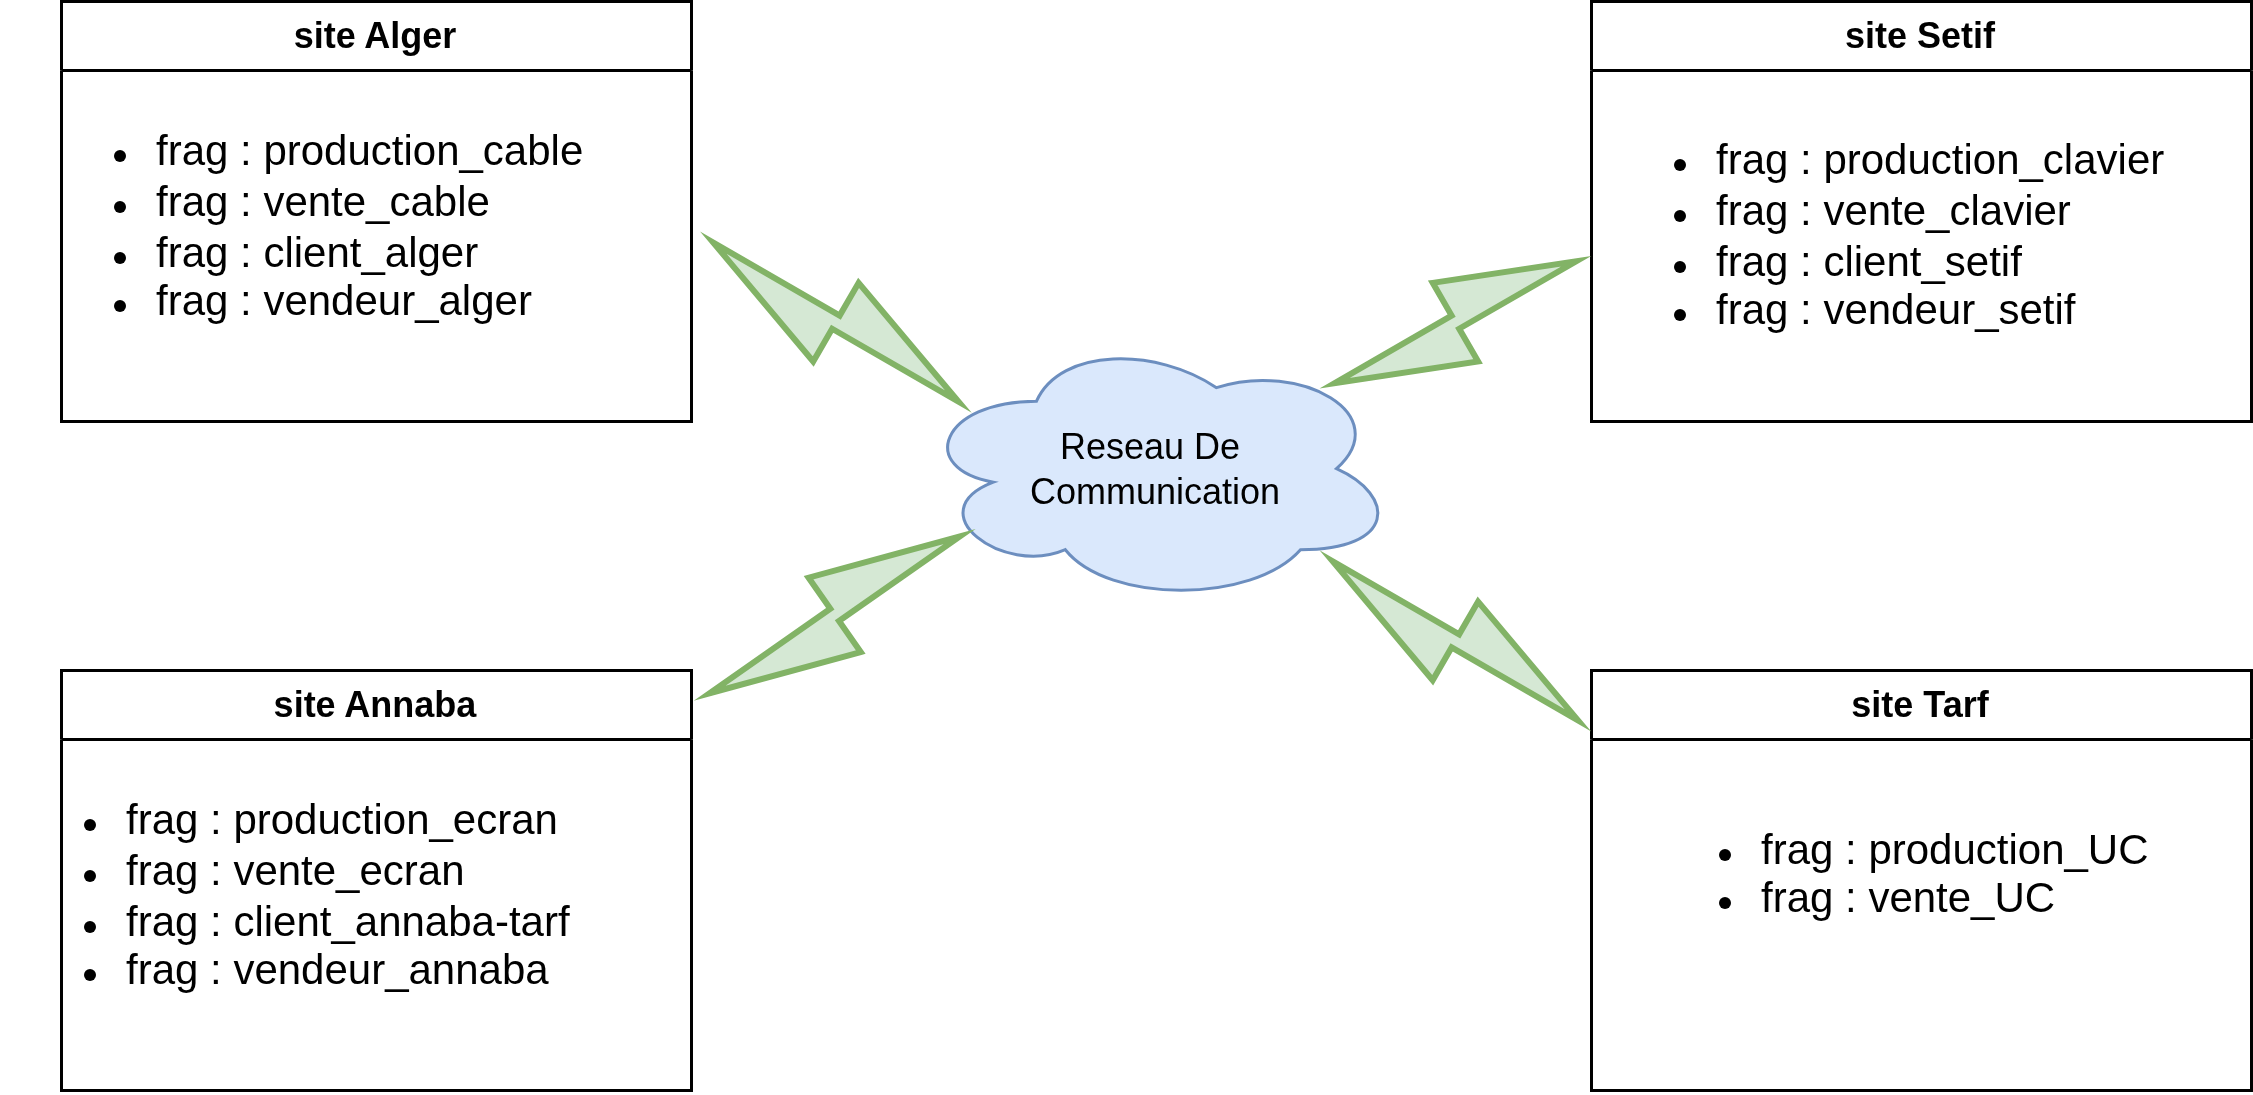
\includegraphics[width=0.55\textwidth]{alloc2.png} 
\end{figure}

\vspace{0.4cm}

R1 : Quelle est la quantité disponible du produit de numéro de série ‘77y6878’.
\begin{codeInput}{sql}{R1}{code01}{41}
SELECT QUANTITE FROM PRODUCTION
WHERE NUMSERIE = '77y6878';
\end{codeInput}

\vspace{0.35cm}
Arbre algebrique global :

\begin{center}
\begin{forest}
    for tree = {align=center , l=1.5cm}
    [$\prod_{\text{Quantite}}$
        [$\sigma_{\text{numserie = '77y678'}}$
            [Production]
    ]
]
\end{forest}
\end{center}

\vspace{0.15cm}
Arbre algebrique canonique (On remplace la table avec ces fragments et on utilise l'operateur de reconstruction $\bigcup$ ) :

\begin{center}
\begin{forest}
for tree = {align=center , l=1.5cm}
[$\prod_{\text{Quantite}}$
    [$\sigma_{\text{numserie = '77y678'}}$
        [$\bigcup$
         [$\text{Production}_{\text{UC}}$]
         [$\text{Production}_{\text{Clavier}}$]
         [$\text{Production}_{\text{Ecran}}$]
         [$\text{Production}_{\text{Cable}}$]
        ]
]
]
\end{forest}
\end{center}

\vspace{0.15cm}
regle optimisation generale (descente des operateurs de reductions de taille projection et restriction avant $\bigcup$) :
\begin{center}
\begin{forest}
for tree = {align=center , l=1.5cm}
[$\bigcup$
         [$\prod_{\text{Quantite}}$
         [$\sigma_{\text{numserie = '77y678'}}$
         [$\text{Production}_{\text{UC}}$]
         ]
         ]
         [$\prod_{\text{Quantite}}$
         [$\sigma_{\text{numserie = '77y678'}}$
         [$\text{Production}_{\text{Clavier}}$]
         ]
         ]
         [$\prod_{\text{Quantite}}$
         [$\sigma_{\text{numserie = '77y678'}}$
         [$\text{Production}_{\text{Ecran}}$]
         ]
         ]
         [$\prod_{\text{Quantite}}$
        [$\sigma_{\text{numserie = '77y678'}}$
         [$\text{Production}_{\text{Cable}}$]
         ]
         ]
        ]
]
\end{forest}
\end{center}

\newpage
R2 : La somme des quantités de produits par composant et modèle.
\begin{codeInput}{sql}{R2}{code01}{41}
SELECT SUM(QUANTITE),COMPOSANT,MODEL FROM PRODUCTION
GROUP BY COMPOSANT,MODEL;
\end{codeInput}


\vspace{0.35cm}
Arbre algebrique global :

\begin{center}
\begin{forest}
    for tree = {align=center , l=1.5cm}
    [$\prod_{\text{sum(Quantite),Composant,Model}}$
            [Production]
]
\end{forest}
\end{center}

\vspace{0.15cm}
Arbre algebrique canonique (On remplace la table avec ces fragments et on utilise l'operateur de reconstruction $\bigcup$ ) :

\begin{center}
\begin{forest}
    for tree = {align=center , l=1.5cm}
    [$\prod_{\text{sum(Quantite),Composant,Model}}$
            [$\bigcup$
         [$\text{Production}_{\text{UC}}$]
         [$\text{Production}_{\text{Clavier}}$]
         [$\text{Production}_{\text{Ecran}}$]
         [$\text{Production}_{\text{Cable}}$]
        ]
]
\end{forest}
\end{center}

\vspace{0.15cm}
regle optimisation generale (descente des operateurs de reductions de taille projection avant $\bigcup$) :

\begin{center}
\begin{forest}
    for tree = {align=center , l=1.5cm, inner sep=1.5pt, font=\small}
            [$\bigcup$
         [$\prod_{\text{sum(Quantite),Composant,Model}}$
         [$\text{Production}_{\text{UC}}$]
         ]
         [$\prod_{\text{sum(Quantite),Composant,Model}}$
         [$\text{Production}_{\text{Clavier}}$]
         ]
         [$\prod_{\text{sum(Quantite),Composant,Model}}$
         [$\text{Production}_{\text{Ecran}}$]
         ]
         [$\prod_{\text{sum(Quantite),Composant,Model}}$
         [$\text{Production}_{\text{Cable}}$]
         ]
        ]
\end{forest}
\end{center}

\vspace{1cm}

\begin{itemize}
    \item \textbf{Stratégie 01} : Envoyer les fragments PROD\_UC, PROD\_CLAVIER et PROD\_CABLE à
Annaba et exécuter la requête.
    \item \textbf{Stratégie 02} : Envoyer les projections sur les attributs modèle et quantité pour chaque
fragments PROD\_UC, PROD\_CLAVIER et PROD\_CABLE à Annaba et
exécuter la requête.
\item \textbf{Stratégie 03} : Calculer la somme des quantités de produits par composant et modèle pour
chaque site et envoyer le résultat à Annaba et exécuter l’union avec le
résultat des composants de Annaba.
\item \textbf{Stratégie 04} : Calculer la somme des quantités de produits par composant et modèle pour
les sites Tarf et Sétif puis envoyer le résultat à Alger et exécuter l’union avec
la somme des quantités de produits par composant et modèle pour site
Alger. Envoyer le résultat à Annaba et faire l’union avec le résultat des
composants de Annaba
\end{itemize}

\newpage
\exer{2}

\vspace{0.25cm}

Fragmentation d'agence :\\[0.1cm]
Puisque l’ecole a trois sites Alger, Constantine, Oran on va effectuer une fragmentation horizontale principale sur l’attribut villeAG.

\begin{alignat*}{2}
    &\text{Agence}_{\text{Alger}} &&= \sigma_{\text{villeAG = 'Alger'}} (\text{Agence})\\[0.1cm]
    &\text{Agence}_{\text{Const}} &&= \sigma_{\text{villeAG = 'Constantine'}} (\text{Agence})\\[0.1cm]
    &\text{Agence}_{\text{Oran}} &&= \sigma_{\text{villeAG = 'Oran'}} (\text{Agence})
\end{alignat*}

\vspace{0.25cm}

Fragmentation de Personnel-Administrative :\\[0.1cm]
Puisque la table possède une clé étrangère \texttt{numAG} qui fait référence à la table agence, déjà fragmentée en
\textbf{FHP}, on va effectuer une fragmentation horizontale dérivée.

\begin{alignat*}{2}
    &\text{P-A}_{\text{Alger}} &&= \text{P-A} \ltimes \text{Agence}_{\text{Alger}}\\[0.1cm]
    &\text{P-A}_{\text{Const}} &&= \text{P-A} \ltimes \text{Agence}_{\text{Const}}\\[0.1cm]
    &\text{P-A}_{\text{Oran}} &&= \text{P-A} \ltimes \text{Agence}_{\text{Oran}}
\end{alignat*}


\vspace{0.25cm}

Fragmentation de Vehicule:\\[0.1cm]
Puisque la table possède une clé étrangère \texttt{numAG} qui fait référence à la table agence, déjà fragmentée en
\textbf{FHP}, on va effectuer une fragmentation horizontale dérivée.

\begin{alignat*}{2}
    &\text{Vehicule}_{\text{Alger}} &&= \text{Vehicule} \ltimes \text{Agence}_{\text{Alger}}\\[0.1cm]
    &\text{Vehicule}_{\text{Const}} &&= \text{Vehicule} \ltimes \text{Agence}_{\text{Const}}\\[0.1cm]
    &\text{Vehicule}_{\text{Oran}} &&= \text{Vehicule} \ltimes \text{Agence}_{\text{Oran}}
\end{alignat*}

\vspace{0.25cm}

Fragmentation de Client:\\[0.1cm]
Puisque la table possède une clé étrangère \texttt{numAG} qui fait référence à la table agence, déjà fragmentée en
\textbf{FHP}, on va effectuer une fragmentation horizontale dérivée.

\begin{alignat*}{2}
    &\text{Client}_{\text{Alger}} &&= \text{Client} \ltimes \text{Agence}_{\text{Alger}}\\[0.1cm]
    &\text{Client}_{\text{Const}} &&= \text{Client} \ltimes \text{Agence}_{\text{Const}}\\[0.1cm]
    &\text{Client}_{\text{Oran}} &&= \text{Client} \ltimes \text{Agence}_{\text{Oran}}
\end{alignat*}


\vspace{0.25cm}
Fragmentation de Cours:\\[0.1cm]
Puisque la table possède une clé étrangère \texttt{numCli} qui fait référence à la table client, déjà fragmentée en
\textbf{FHP}, on va effectuer une fragmentation horizontale dérivée.

\begin{alignat*}{2}
    &\text{Cours}_{\text{Alger}} &&= \text{Cours} \ltimes \text{Client}_{\text{Alger}}\\[0.1cm]
    &\text{Cours}_{\text{Const}} &&= \text{Cours} \ltimes \text{Client}_{\text{Const}}\\[0.1cm]
    &\text{Cours}_{\text{Oran}} &&= \text{Cours} \ltimes \text{Client}_{\text{Oran}}
\end{alignat*}



\vspace{0.25cm}
Fragmentation d'Examen:\\[0.1cm]
Puisque la table possède une clé étrangère \texttt{numCli} qui fait référence à la table client, déjà fragmentée en
\textbf{FHP}, on va effectuer une fragmentation horizontale dérivée.

\begin{alignat*}{2}
    &\text{Examen}_{\text{Alger}} &&= \text{Examen} \ltimes \text{Client}_{\text{Alger}}\\[0.1cm]
    &\text{Examen}_{\text{Const}} &&= \text{Examen} \ltimes \text{Client}_{\text{Const}}\\[0.1cm]
    &\text{Examen}_{\text{Oran}} &&= \text{Examen} \ltimes \text{Client}_{\text{Oran}}
\end{alignat*}




\newpage
Autre fragmentation possible pour vehicule et cours :
\begin{itemize}
    \item vehicule on peut faire une \textbf{FHD} avec P-A grace a la cle etrangere \texttt{num-Instructeur}.
    \item Cours on peut faire une \textbf{FHD} avec Vehicule grace a la cle etrangere \texttt{numV} , ou une \textbf{FHD}
        avec P-A grace a la cle etrangere \texttt{num-Instructeur}.
\end{itemize}

\vspace{0.15cm}
Toute les fragmentations donne le meme resultat 2 fragment Alger Constantine Oran car il sont tous des \textbf{FHD} de 
table qui on ete fragmente de la meme maniere par rapport a la ville.
\vspace{0.4cm}

\begin{codeInput}{sql}{Fragmentation}{code01}{41}
-- FHP
CREATE TABLE AGENCE (
    NUMAG INT,
    VILLEAG VARCHAR2(50),
    NUM-GERANT INT,
    NBR-INSTRUCTEURS INT,
    CONSTRAINT PK_AGENCE PRIMARY KEY (NUMAG),
    CONSTRAINT FK_AGENCE_PA FOREIGN KEY (NUM-GERANT) REFERENCES PA(NUMP)
 )
 PARTITION BY LIST (VILLEAG) (
    PARTITION AGENCE_ALGER VALUES ('ALGER'),
    PARTITION AGENCE_CONST VALUES ('CONSTANTINE'),
    PARTITION AGENCE_ORAN VALUES('ORAN') 
 );

-- FHD
CREATE TABLE CLIENT (
    NUMCLI INT,
    NOMCLI VARCHAR2(50),
    ADRESSECLI VARCHAR2(100),
    NUMAG INT,
    AGE INT,
    CONSTRAINT PK_CLIENT PRIMARY KEY (NUMCLI),
    CONSTRAINT FK_CLIENT_AGENCE FOREIGN KEY (NUMAG) REFERENCES AGENCE(NUMAG))
PARTITION BY REFERENCE (FK_CLIENT_AGENCE);
\end{codeInput}

\vspace{0.75cm}

Schéma d'allocation :

\begin{figure}[H] 
  \centering 
  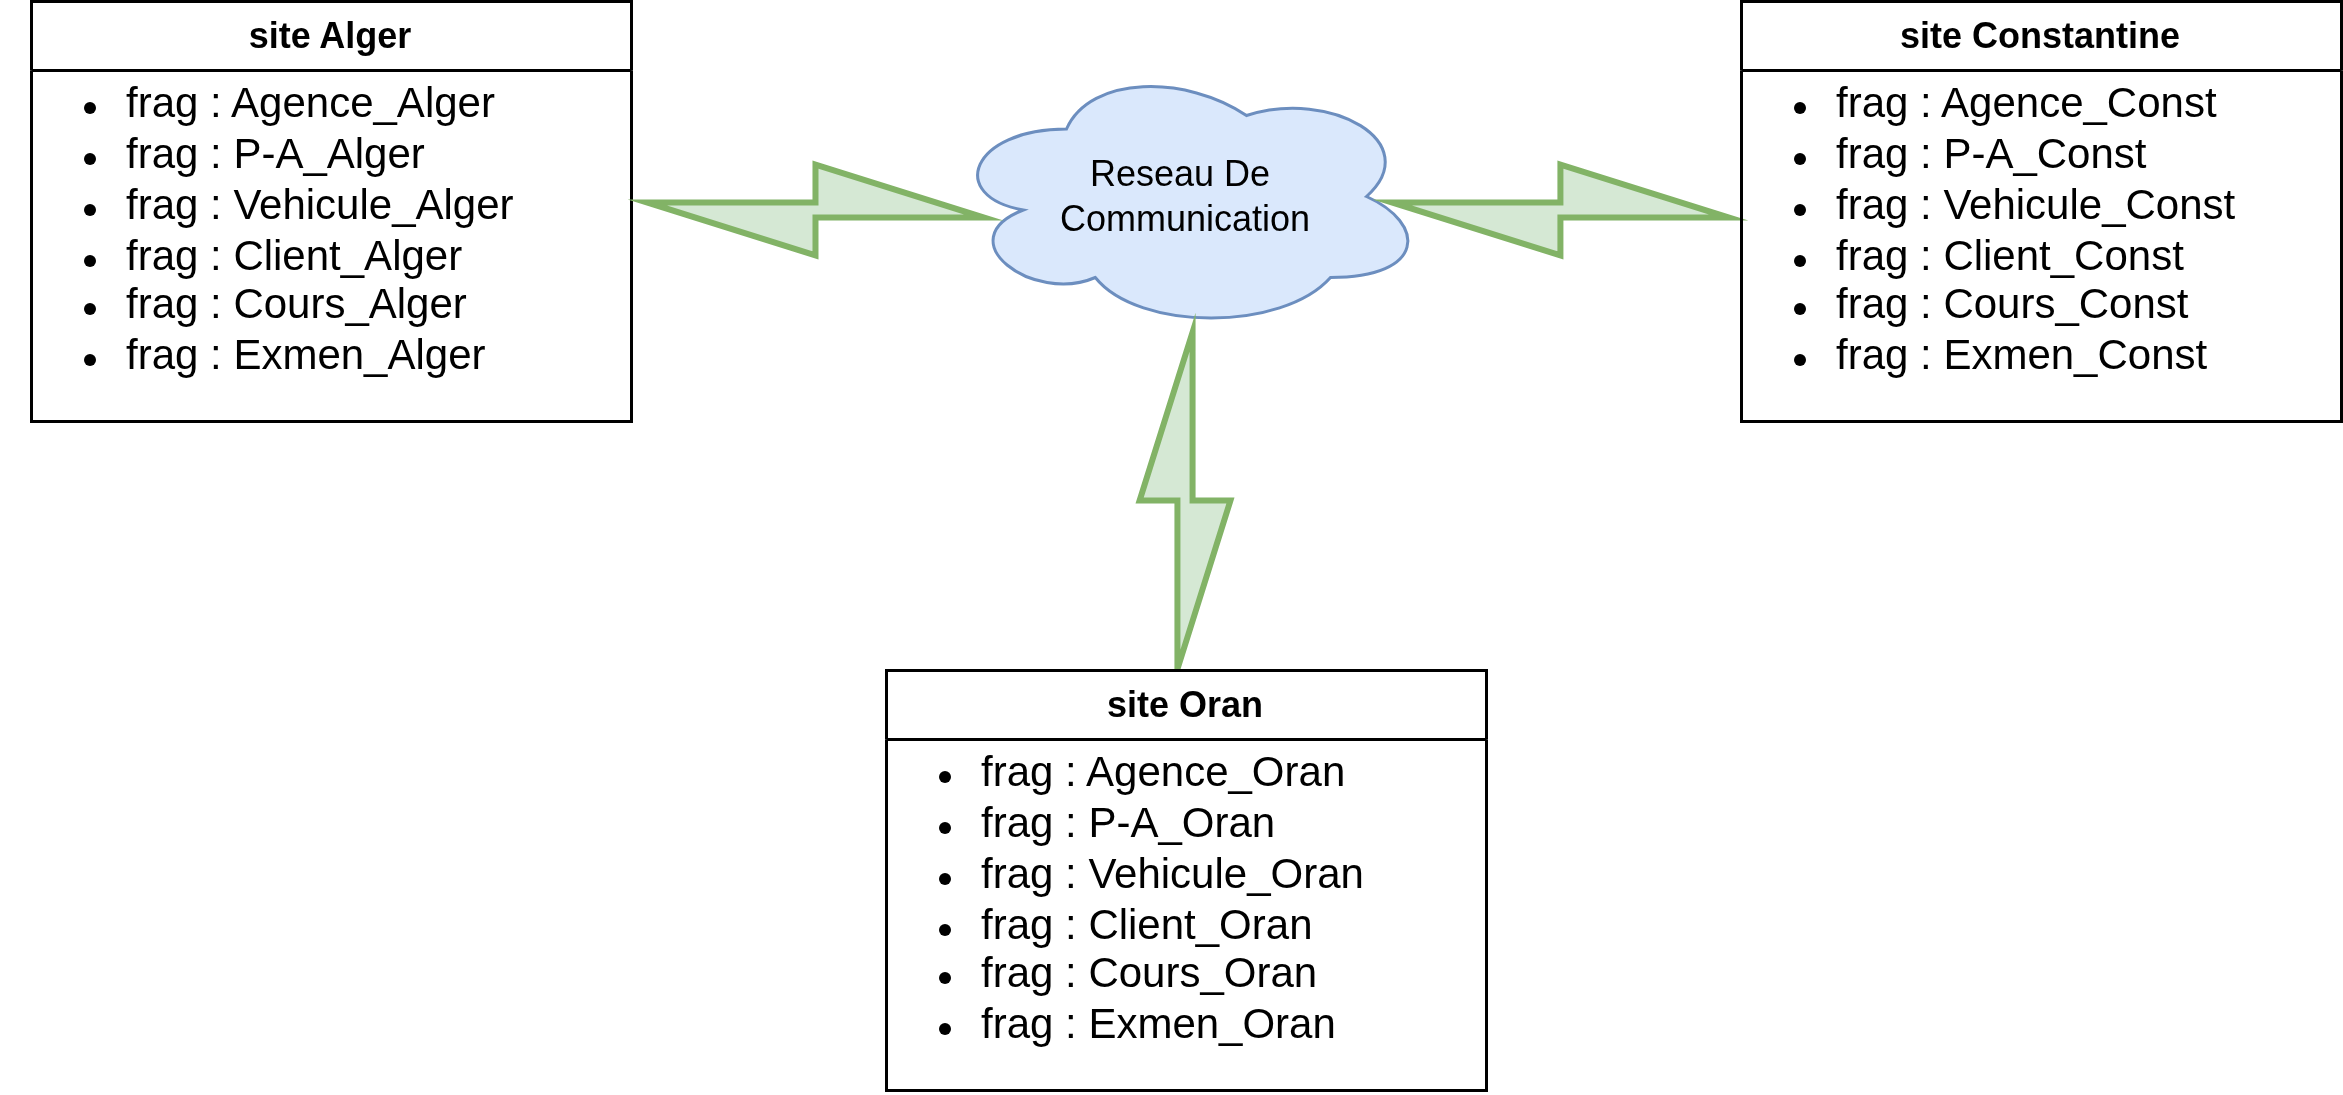
\includegraphics[width=0.55\textwidth]{alloc3.png} 
\end{figure}


\vspace{0.3cm}
On met une copie du fragment $\text{vehicule}_{\text{Alger}}$ dans le site Oran 
mais il foudra synchronizer le fragment entre alger and oran quand il ya un changement.

\newpage

R : Donner les nom et numéro de tous les clients de moins de 25 ans, relevant des agences d'Alger ou d'Oran, qui ont eu un 
résultat positif à l'examen du 22/05/2019
\begin{codeInput}{sql}{R}{code01}{41}
SELECT C.NOMCLI , C.NUMCLI FROM CLIENT C, AGENCE A, EXAMEN E 
WHERE A.VILLEAG IN ('Alger','Oran') AND C.AGE < 25 AND E.DATE-EXAMEN = '22/05/2019' AND 
E.RESULTAT='POSITIVE' AND C.NUMAG = A.NUMAG AND C.NUMCLI = E.NUMCLI; 
\end{codeInput}


\vspace{0.35cm}
Arbre algebrique global :

\begin{center}
\begin{forest}
    for tree = {align=center , l=1.5cm}
    [$\prod_{\text{nomcli,numcli}}$
        [$\sigma_{\text{villeAG in ('Alger','Oran') and age} < \text{25 and date} < \text{'22/05/2019' and resultat = 'Positive'}}$
        [$\displaystyle \JoinOp^{\text{numCli}}$
        [$\displaystyle \JoinOp^{\text{numAG}}$
                [Agence , tier = leaf]
                [Client , tier = leaf]
            ]
            [Examen , tier = leaf]
            ]
            ]
]
\end{forest}
\end{center}


\vspace{0.15cm}
Arbre algebrique canonique (On remplace la table avec ces fragments et on utilise l'operateur de reconstruction $\bigcup$ ) :

\begin{center}
\begin{forest}
    for tree = {
        align=center, 
        l=1.5cm, 
        inner sep=1.5pt, 
        font=\small,
        s sep=5pt 
    }
    [{$\prod_{\text{nomcli,numcli}}$}
        [{$\sigma_{\text{villeAG in ('Alger','Oran') and age} < \text{25 and date} < \text{'22/05/2019' and resultat = 'Positive'}}$}
            [$\displaystyle \JoinOp^{\text{numCli}}$
                [$\displaystyle \JoinOp^{\text{numAG}}$
                    [$\bigcup$
                        [$\text{Agence}_{\text{Alger}}$, tier=leaf]
                        [$\text{Agence}_{\text{Oran}}$, tier=leaf]
                        [$\text{Agence}_{\text{Const}}$, tier=leaf]
                    ]
                    [$\bigcup$
                        [$\text{Client}_{\text{Alger}}$, tier=leaf]
                        [$\text{Client}_{\text{Oran}}$, tier=leaf]
                        [$\text{Client}_{\text{Const}}$, tier=leaf]
                    ]
                ]
                [$\bigcup$
                    [$\text{Examen}_{\text{Alger}}$, tier=leaf]
                    [$\text{Examen}_{\text{Oran}}$, tier=leaf]
                    [$\text{Examen}_{\text{Const}}$, tier=leaf]
                ]
            ]
        ]
    ]
\end{forest}
\end{center}

\newpage

regle optimisation generale (descente des operateurs de reductions de taille restriction avant $\bigcup$) :

\begin{center}
\resizebox{\textwidth}{!}{%
\begin{forest}
    for tree = {
        align=center, 
        l=1.5cm, 
        inner sep=1.5pt, 
        font=\small,
        s sep=5pt 
    }
    [{$\prod_{\text{nomcli,numcli}}$}
            [$\displaystyle \JoinOp^{\text{numCli}}$
                [$\displaystyle \JoinOp^{\text{numAG}}$
                    [$\bigcup$
                    [\textcolor{blue}{$\sigma_{\text{villeAG in ('Alger','Oran')}}$}
                    [\textcolor{blue}{$\text{Agence}_{\text{Alger}}$}, tier=leaf,edge={blue}]
                        ]
                        [\textcolor{blue}{$\sigma_{\text{villeAG in ('Alger','Oran')}}$}
                        [\textcolor{blue}{$\text{Agence}_{\text{Oran}}$}, tier=leaf, edge={blue}]
                        ]
                        [\textcolor{red}{$\sigma_{\text{villeAG in ('Alger','Oran')}}$}
                        [\textcolor{red}{$\text{Agence}_{\text{Const}}$}, tier=leaf, edge={red}]
                        ]
                    ]
                    [$\bigcup$
                        [$\sigma_{\text{age} <25}$
                        [$\text{Client}_{\text{Alger}}$, tier=leaf]
                        ]
                        [$\sigma_{\text{age} <25}$
                        [$\text{Client}_{\text{Oran}}$, tier=leaf]
                        ]
                        [$\sigma_{\text{age} <25}$
                        [$\text{Client}_{\text{Const}}$, tier=leaf]
                        ]
                    ]
                ]
                [$\bigcup$
                    [$\sigma_{\text{date} < \text{'22/05/2019' and resultat = 'Positive'}}$
                    [$\text{Examen}_{\text{Alger}}$, tier=leaf]
                    ]
                    [$\sigma_{\text{date} < \text{'22/05/2019' and resultat = 'Positive'}}$
                    [$\text{Examen}_{\text{Oran}}$, tier=leaf]
                    ]
                    [$\sigma_{\text{date} < \text{'22/05/2019' and resultat = 'Positive'}}$
                    [$\text{Examen}_{\text{Const}}$, tier=leaf]
                    ]
                ]
            ]
    ]
\end{forest}%
}
\end{center}

\vspace{0.25cm}

Suppression de \textcolor{red}{fragment vide} et \textcolor{blue}{restriction inutile}: 


\begin{center}
\resizebox{\textwidth}{!}{%
\begin{forest}
    for tree = {
        align=center, 
        l=1.5cm, 
        inner sep=1.5pt, 
        font=\small,
        s sep=5pt 
    }
    [{$\prod_{\text{nomcli,numcli}}$}
            [$\displaystyle \JoinOp^{\text{numCli}}$
                [$\displaystyle \JoinOp^{\text{numAG}}$
                    [$\bigcup$
                    [$\text{Agence}_{\text{Alger}}$, tier=leaf]
                    [$\text{Agence}_{\text{Oran}}$, tier=leaf]
                    ]
                    [$\bigcup$
                        [$\sigma_{\text{age} <25}$
                        [$\text{Client}_{\text{Alger}}$, tier=leaf]
                        ]
                        [$\sigma_{\text{age} <25}$
                        [$\text{Client}_{\text{Oran}}$, tier=leaf]
                        ]
                        [$\sigma_{\text{age} <25}$
                        [$\text{Client}_{\text{Const}}$, tier=leaf]
                        ]
                    ]
                ]
                [$\bigcup$
                    [$\sigma_{\text{date} < \text{'22/05/2019' and resultat = 'Positive'}}$
                    [$\text{Examen}_{\text{Alger}}$, tier=leaf]
                    ]
                    [$\sigma_{\text{date} < \text{'22/05/2019' and resultat = 'Positive'}}$
                    [$\text{Examen}_{\text{Oran}}$, tier=leaf]
                    ]
                    [$\sigma_{\text{date} < \text{'22/05/2019' and resultat = 'Positive'}}$
                    [$\text{Examen}_{\text{Const}}$, tier=leaf]
                    ]
                ]
            ]
    ]
\end{forest}%
}
\end{center}

\vspace{0.25cm}
Distribution de la jointure par rapport à l’union et élimination des fragments vides :\\[0.1cm]
On met $\text{Agence}_{\text{Alger}} : A_1$ , $\text{Agence}_{\text{Oran}} : A_2$ , $\text{Client}_{\text{Alger}} : C_1$ 
,  $\text{Client}_{\text{Oran}} : C_2$ ,  $\text{Client}_{\text{Const}} : C_3$ .

\begin{align*}
    (A_1 \bigcup A_2) \bowtie (C_1 \bigcup C_2 \bigcup C_3) &= (A_1 \bowtie C_1) \bigcup \underbrace{(A_1 \bowtie C_2)}_{\emptyset} \bigcup \underbrace{(A_1 \bowtie C_3)}_{\emptyset} \bigcup \underbrace{(A_2 \bowtie C_1)}_{\emptyset} \bigcup (A_2 \bowtie C_2) \bigcup \underbrace{(A_2 \bowtie C_3)}_{\emptyset}\\[0.1cm]
                                                            &= (A_1 \bowtie C_1) \bigcup (A_2 \bowtie C_2)
\end{align*}


\begin{center}
\resizebox{\textwidth}{!}{%
\begin{forest}
    for tree = {
        align=center, 
        l=1.5cm, 
        inner sep=1.5pt, 
        font=\small,
        s sep=5pt 
    }
    [{$\prod_{\text{nomcli,numcli}}$}
            [$\displaystyle \JoinOp^{\text{numCli}}$
                [$\bigcup$
                [$\displaystyle \JoinOp^{\text{numAG}}$
                    [$\text{Agence}_{\text{Alger}}$, tier=leaf]
                    [$\sigma_{\text{age} <25}$
                    [$\text{Client}_{\text{Alger}}$, tier=leaf]
                    ]
                    ]
                    [$\displaystyle \JoinOp^{\text{numAG}}$
                    [$\text{Agence}_{\text{Oran}}$, tier=leaf]
                        [$\sigma_{\text{age} <25}$
                        [$\text{Client}_{\text{Oran}}$, tier=leaf]
                        ]
                    ]
                ]
                [$\bigcup$
                    [$\sigma_{\text{date} < \text{'22/05/2019' and resultat = 'Positive'}}$
                    [$\text{Examen}_{\text{Alger}}$, tier=leaf]
                    ]
                    [$\sigma_{\text{date} < \text{'22/05/2019' and resultat = 'Positive'}}$
                    [$\text{Examen}_{\text{Oran}}$, tier=leaf]
                    ]
                    [$\sigma_{\text{date} < \text{'22/05/2019' and resultat = 'Positive'}}$
                    [$\text{Examen}_{\text{Const}}$, tier=leaf]
                    ]
                ]
            ]
    ]
\end{forest}%
}
\end{center}

\newpage

Distribution de la jointure par rapport à l’union et élimination des fragments vides, descente des operateurs de reductions de taille projection avant $\bigcup$  :\\[0.1cm]
On met $(A_1 \bowtie C_1) : AC_1$ , $(A_2 \bowtie C_2) : AC_2$ , $\text{Examen}_{\text{Alger}} : E_1$ 
,  $\text{Examen}_{\text{Oran}} : E_2$ ,  $\text{Examen}_{\text{Const}} : E_3$ .

\begin{align*}
    (AC_1 \bigcup AC_2) \bowtie (E_1 \bigcup E_2 \bigcup E_3) &= (AC_1 \bowtie E_1) \bigcup \underbrace{(AC_1 \bowtie E_2)}_{\emptyset} \bigcup \underbrace{(AC_1 \bowtie E_3)}_{\emptyset} \bigcup \underbrace{(AC_2 \bowtie E_1)}_{\emptyset} \bigcup (AC_2 \bowtie E_2) \bigcup \underbrace{(AC_2 \bowtie E_3)}_{\emptyset}\\[0.1cm]
                                                            &= (AC_1 \bowtie E_1) \bigcup (AC_2 \bowtie E_2)
\end{align*}


\begin{center}
\resizebox{\textwidth}{!}{%
\begin{forest}
    for tree = {
        align=center, 
        l=1.5cm, 
        inner sep=1.5pt, 
        font=\small,
        s sep=5pt 
    }
                [$\bigcup$
    [$\prod_{\text{nomcli,numcli}}$
            [$\displaystyle \JoinOp^{\text{numCli}}$
                [$\displaystyle \JoinOp^{\text{numAG}}$
                    [$\text{Agence}_{\text{Alger}}$, tier=leaf]
                    [$\sigma_{\text{age} <25}$
                    [$\text{Client}_{\text{Alger}}$, tier=leaf]
                    ]
                    ]
                    [$\sigma_{\text{date} < \text{'22/05/2019' and resultat = 'Positive'}}$
                    [$\text{Examen}_{\text{Alger}}$, tier=leaf]
                    ]
                ]
                ]
    [$\prod_{\text{nomcli,numcli}}$
            [$\displaystyle \JoinOp^{\text{numCli}}$
                    [$\displaystyle \JoinOp^{\text{numAG}}$
                    [$\text{Agence}_{\text{Oran}}$, tier=leaf]
                        [$\sigma_{\text{age} <25}$
                        [$\text{Client}_{\text{Oran}}$, tier=leaf]
                        ]
                    ]
                    [$\sigma_{\text{date} < \text{'22/05/2019' and resultat = 'Positive'}}$
                    [$\text{Examen}_{\text{Oran}}$, tier=leaf]
                    ]
                ]
                ]
            ]
    
\end{forest}%
}
\end{center}

\vspace{1cm}

\begin{itemize}
    \item \textbf{Stratégie1} :Exécuter la partie gauche de l’arbre précédent à Alger
Exécuter la partie droite à Oran et envoyer le résultat à Alger
Faire l’union des deux résultats
\item \textbf{Stratégie 2} :Envoyer les fragments Agence\_Oran, Client\_Oran et
Examen\_Oran à Alger
Exécuter toute la requête sur Alger
\end{itemize}

\newpage
\exer{3}

\vspace{0.15cm}
On a
\begin{codeInput}{sql}{R}{code01}{41}
-- R1 
SELECT NOM,PRENOM,EMAIL FROM UTILISATEUR WHERE DATE_DERNIER_ACCES < '01-03-2011';

-- R2
SELECT VILLE,PAYS,AGE FROM UTILISATEUR WHERE DATE_ENREGISTREMENT < '01-01-2011';

-- R3 
SELECT NOM,PRENOM,VILLE FROM UTILISATEUR WHERE AGE > 18;
\end{codeInput}

\vspace{0.35cm}

User1 aura besoin de l'attribut cle primaire IDU , les attributs selectioner dans la requete R1 (NOM,PRENOM,EMAIL) et
l'attribut dans la condition where (DATE\_DERNIER\_ACCESS) :
\[\text{User1} = \textstyle \prod_{\text{IDU,NOM,PRENOM,EMAIL,DATE\_DERNIER\_ACCESS}} (\text{Utilisateur})\]

\vspace{0.25cm}


User2 aura besoin de l'attribut cle primaire IDU , les attributs selectioner dans la requete R2 (VILLE,PAYS,AGE) et
l'attribut dans la condition where (DATE\_ENREGISTREMENT) :
\[\text{User2} = \textstyle \prod_{\text{IDU,VILLE,PAYS,AGE,DATE\_ENREGISTREMENT}} (\text{Utilisateur})\]

\vspace{0.25cm}


User3 aura besoin de l'attribut cle primaire IDU , les attributs restants (MOT\_DE\_PASSE,CODE\_POSTAL,TELEPHONE): 
\[\text{User3} = \textstyle \prod_{\text{IDU,MOT\_DE\_PASSE,CODE\_POSTAL,TELEPHONE}} (\text{Utilisateur})\]

\vspace{0.5cm}
R1\\
Arbre algebrique global :

\begin{center}
\begin{forest}
    for tree = {align=center , l=1.5cm}
    [$\prod_{\text{nom,prenom,email}}$
[$\sigma_{\text{date\_dernier\_access} < \text{'01-03-2011'}}$
            [Utilisateur]
    ]
]
\end{forest}
\end{center}

\vspace{0.4cm}
Arbre algebrique Canonique on remplace la table avec ces fragments et on utilise l'operateur de reconstruction $\bowtie$:

\begin{center}
\begin{forest}
    for tree = {align=center , l=1.5cm}
    [$\prod_{\text{nom,prenom,email}}$
[$\sigma_{\text{date\_dernier\_access} < \text{'01-03-2011'}}$
        [$\displaystyle \JoinOp^{\text{IDU}}$
        [$\displaystyle \JoinOp^{\text{IDU}}$
        [User1,tier=leaf]
        [User2,tier=leaf]
        ]
        [User3,tier=leaf]
        ]
    ]
]
\end{forest}
\end{center}

\newpage
Optimisation General descente des operateur de reduction de taille projection, reduction :


\begin{center}
\begin{forest}
    for tree = {align=center , l=1.5cm}
    [$\prod_{\text{nom,prenom,email}}$
        [$\displaystyle \JoinOp^{\text{IDU}}$
        [$\prod_{\text{IDU,nom,prenom,email}}$
        [$\displaystyle \JoinOp^{\text{IDU}}$
        [$\prod_{\text{IDU,nom,prenom,email}}$
        [$\sigma_{\text{date\_dernier\_access} < \text{'01-03-2011'}}$
        [User1,tier=leaf]
        ]
        ]
        [\textcolor{red}{$\prod_{\text{IDU,nom,prenom,email}}$}
        [\textcolor{red}{User2},tier=leaf,edge={red}]
        ]
        ]
        ]
        [\textcolor{red}{$\prod_{\text{IDU,nom,prenom,email}}$}
        [\textcolor{red}{User3},tier=leaf,edge={red}]
        ]
        ]
]
\end{forest}
\end{center}

\vspace{0.4cm}

Supression \textcolor{red}{des fragments vide} :

\begin{center}
\begin{forest}
    for tree = {align=center , l=1.5cm}
    [$\prod_{\text{nom,prenom,email}}$
    [\textcolor{blue}{$\prod_{\text{IDU,nom,prenom,email}}$},edge={blue}
        [$\sigma_{\text{date\_dernier\_access} < \text{'01-03-2011'}}$
        [User1,tier=leaf]
        ]
        ]
        ]
\end{forest}
\end{center}


\vspace{0.4cm}

Supression \textcolor{blue}{projection inutile} :

\begin{center}
\begin{forest}
    for tree = {align=center , l=1.5cm}
    [$\prod_{\text{nom,prenom,email}}$
        [$\sigma_{\text{date\_dernier\_access} < \text{'01-03-2011'}}$
        [User1,tier=leaf]
        ]
        ]
\end{forest}
\end{center}

\vspace{0.25cm}

\begin{codeInput}{sql}{R1}{code01}{41}
SELECT NOM,PRENOM,EMAIL FROM USER1 WHERE DATE_DERNIER_ACCES < '01-03-2011';
\end{codeInput}


\newpage
R2\\
Arbre algebrique global :

\begin{center}
\begin{forest}
    for tree = {align=center , l=1.5cm}
    [$\prod_{\text{ville,pays,age}}$
[$\sigma_{\text{date\_enregistrement} < \text{'01-01-2011'}}$
            [Utilisateur]
    ]
]
\end{forest}
\end{center}

\vspace{0.4cm}
Arbre algebrique Canonique on remplace la table avec ces fragments et on utilise l'operateur de reconstruction $\bowtie$:

\begin{center}
\begin{forest}
    for tree = {align=center , l=1.5cm}
    [$\prod_{\text{ville,pays,age}}$
[$\sigma_{\text{date\_enregistrement} < \text{'01-01-2011'}}$
        [$\displaystyle \JoinOp^{\text{IDU}}$
        [$\displaystyle \JoinOp^{\text{IDU}}$
        [User1,tier=leaf]
        [User2,tier=leaf]
        ]
        [User3,tier=leaf]
        ]
    ]
]
\end{forest}
\end{center}

\vspace{0.4cm}
Optimisation General descente des operateur de reduction de taille projection, reduction :

\begin{center}
\begin{forest}
    for tree = {align=center , l=1.5cm}
    [$\prod_{\text{ville,pays,age}}$
        [$\displaystyle \JoinOp^{\text{IDU}}$
        [$\prod_{\text{IDU,ville,pays,age}}$
        [$\displaystyle \JoinOp^{\text{IDU}}$
        [\textcolor{red}{$\prod_{\text{IDU,ville,pays,age}}$}
        [\textcolor{red}{User1},tier=leaf,edge={red}]
        ]
        [$\prod_{\text{IDU,ville,pays,age}}$
        [$\sigma_{\text{date\_enregistrement} < \text{'01-01-2011'}}$
        [User2,tier=leaf]
        ]
        ]
        ]
        ]
        [\textcolor{red}{$\prod_{\text{IDU,ville,pays,age}}$}
        [\textcolor{red}{User3},tier=leaf,edge={red}]
        ]
        ]
]
\end{forest}
\end{center}

\newpage

Supression \textcolor{red}{des fragments vide} :


\begin{center}
\begin{forest}
    for tree = {align=center , l=1.5cm}
    [$\prod_{\text{ville,pays,age}}$
    [\textcolor{blue}{$\prod_{\text{IDU,ville,pays,age}}$}, edge={blue}
        [$\sigma_{\text{date\_enregistrement} < \text{'01-01-2011'}}$
        [User2,tier=leaf]
        ]
        ]
]
\end{forest}
\end{center}
\vspace{0.4cm}

Supression \textcolor{blue}{projection inutile} :

\begin{center}
\begin{forest}
    for tree = {align=center , l=1.5cm}
    [$\prod_{\text{ville,pays,age}}$
        [$\sigma_{\text{date\_enregistrement} < \text{'01-01-2011'}}$
        [User2,tier=leaf]
        ]
]
\end{forest}
\end{center}

\vspace{0.25cm}

\begin{codeInput}{sql}{R2}{code01}{41}
SELECT VILLE,PAYS,AGE FROM USER2 WHERE DATE_ENREGISTREMENT < '01-01-2011';
\end{codeInput}

\vspace{0.4cm}
R3\\
Arbre algebrique global :

\begin{center}
\begin{forest}
    for tree = {align=center , l=1.5cm}
    [$\prod_{\text{nom,prenom,ville}}$
[$\sigma_{\text{age} > 18}$
            [Utilisateur]
    ]
]
\end{forest}
\end{center}

\vspace{0.4cm}
Arbre algebrique Canonique on remplace la table avec ces fragments et on utilise l'operateur de reconstruction $\bowtie$:

\begin{center}
\begin{forest}
    for tree = {align=center , l=1.5cm}
    [$\prod_{\text{nom,prenom,ville}}$
[$\sigma_{\text{age} > 18}$
        [$\displaystyle \JoinOp^{\text{IDU}}$
        [$\displaystyle \JoinOp^{\text{IDU}}$
        [User1,tier=leaf]
        [User2,tier=leaf]
        ]
        [User3,tier=leaf]
        ]
    ]
]
\end{forest}
\end{center}

\vspace{0.4cm}
Optimisation General descente des operateur de reduction de taille projection, reduction :



\begin{center}
\begin{forest}
    for tree = {align=center , l=1.5cm}
    [$\prod_{\text{nom,prenom,ville}}$
        [$\displaystyle \JoinOp^{\text{IDU}}$
        [$\prod_{\text{IDU,nom,prenom,ville}}$
        [$\displaystyle \JoinOp^{\text{IDU}}$
        [$\prod_{\text{IDU,nom,prenom}}$
        [User1,tier=leaf]
        ]
        [$\prod_{\text{IDU,ville}}$
        [$\sigma_{\text{age} > 18}$
        [User2,tier=leaf]
        ]
        ]
        ]
        ]
        [\textcolor{red}{$\prod_{\text{IDU,nom,prenom,ville}}$}
        [\textcolor{red}{User3},tier=leaf,edge={red}]
        ]
        ]
]
\end{forest}
\end{center}

\vspace{0.4cm}

Supression \textcolor{red}{des fragments vide} :



\begin{center}
\begin{forest}
    for tree = {align=center , l=1.5cm}
    [$\prod_{\text{nom,prenom,ville}}$
    [\textcolor{blue}{$\prod_{\text{IDU,nom,prenom,ville}}$},egde = {blue}
        [$\displaystyle \JoinOp^{\text{IDU}}$
        [$\prod_{\text{IDU,nom,prenom}}$
        [User1,tier=leaf]
        ]
        [$\prod_{\text{IDU,ville}}$
        [$\sigma_{\text{age} > 18}$
        [User2,tier=leaf]
        ]
        ]
        ]
        ]
]
\end{forest}
\end{center}

\newpage

Supression \textcolor{blue}{projection inutile} :

\begin{center}
\begin{forest}
    for tree = {align=center , l=1.5cm}
    [$\prod_{\text{nom,prenom,ville}}$
        [$\displaystyle \JoinOp^{\text{IDU}}$
        [$\prod_{\text{IDU,nom,prenom}}$
        [User1,tier=leaf]
        ]
        [$\prod_{\text{IDU,ville}}$
        [$\sigma_{\text{age} > 18}$
        [User2,tier=leaf]
        ]
        ]
        ]
]
\end{forest}
\end{center}\vspace{0.25cm}

\begin{codeInput}{sql}{R3}{code01}{41}
SELECT NOM,PRENOM,VILLE FROM USER2,USER1 WHERE AGE > 18 AND USER1.IDU=USER2.IDU;
\end{codeInput}

\vspace{0.15cm}

\begin{prettyBox}{Conclusion}{red}
Les deux requêtes R1 et R2 sont réécrites chacune sur un fragment
car tous les attributs référencés par chacune des requêtes
appartiennent au même fragment. La requête R3 accède à deux
fragments, alors une opération de jointure supplémentaire entre
USER1 et USER2 est ajoutée à la requête pour récupérer tous les
attributs référencés
\end{prettyBox}

\newpage
\exer{4}
\vspace{0.15cm}
\begin{figure}[H] 
  \centering 
  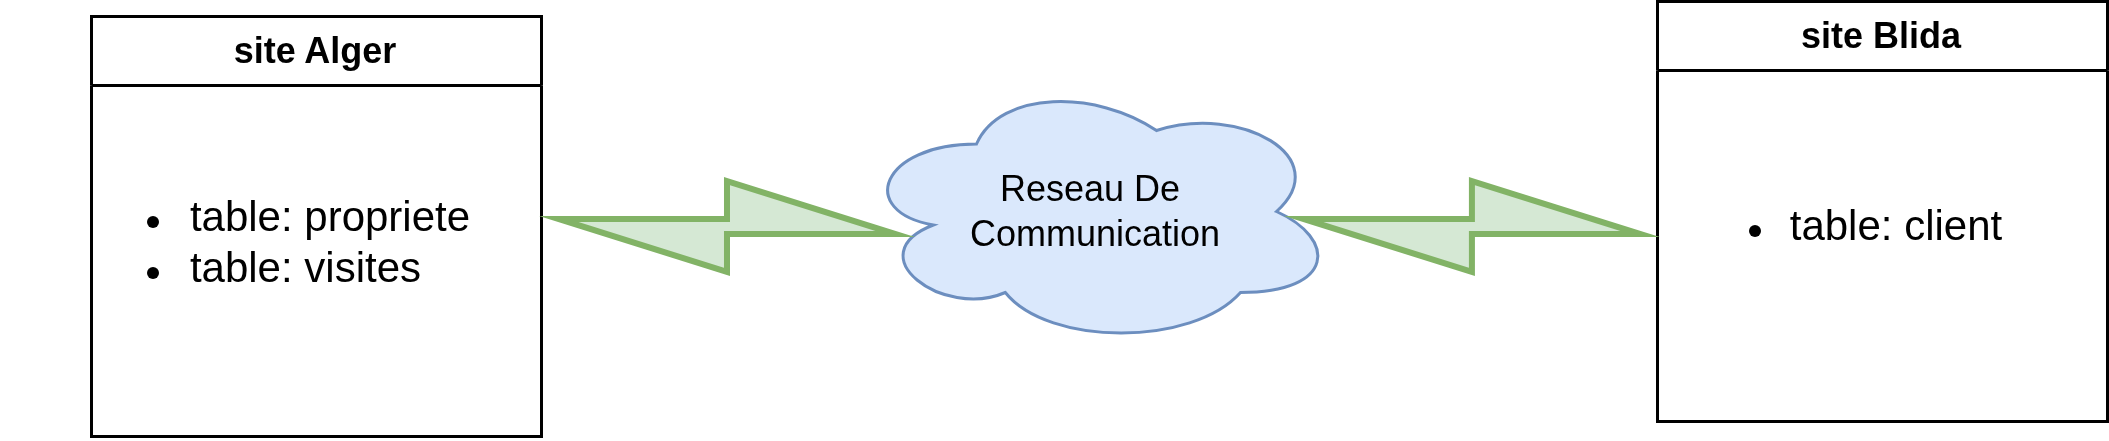
\includegraphics[width=0.65\textwidth]{alloc4.png} 
\end{figure}

\vspace{0.4cm}

\textbf{Stratégie 1} : Déplacer la relation client à Alger et y traiter la
requête.

\begin{align*}
    \text{temp}_{\text{envoie-Client}} &= \text{delai}_{\text{client}} + \dfrac{\text{taille = } \text{nb tuple}_{\text{client}} \cdot \text{ taille tuple}}{\text{taux-transmission}}\\[0.15cm]
                                   &= 1 + \dfrac{10^5 \cdot 10^2}{10^4} \\[0.15cm]
                                   &= 1 + 10^3 = 1001 \text{ s}\\[0.15cm]
                                   &= \dfrac{1001}{60} = 16.68 \text{ min}
\end{align*}

\vspace{0.35cm}
\textbf{Stratégie 2} : Déplacer les relations propriété et visite à Blida et y traiter la requête


\small 
\begin{align*}
    \text{temp}_{\text{envoie-Propriete}} + \text{temp}_{\text{envoie-Visites}}  &= \text{delai}_{\text{Propriete}} + \dfrac{\text{nb tuple}_{\text{propriete}} \cdot \text{taille tuple}}{\text{taux-transmission}} + \text{delai}_{\text{visites}} + \dfrac{\text{nb tuple}_{\text{visites}} \cdot \text{taille tuple}}{\text{taux-transmission}}\\[0.15cm]
                                   &= 1 + \dfrac{10^4 \cdot 10^2}{10^4} + 1 + \dfrac{10^6 \cdot 10^2}{10^4}  \\[0.15cm]
                                   &= 2 + 10^2 + 10^4 = 10102 \text{ s}\\[0.15cm]
                                   &= \dfrac{10102}{3600} = 2.8 \text{ h}
\end{align*}

\vspace{0.35cm}
\textbf{Stratégie 3} : joindre les deux relations propriété et visite à Alger et pour
chaque tuple du résultat vérifier à Blida si le prix max est supérieur à
30 000. La vérification de chaque tuple suppose deux messages : l‘envoi
d’un tuple et une réponse

\small 
\begin{align*}
    \text{temp}_{\text{envoie-joinTuple}} + \text{temp}_{\text{envoie-reponse}}  &= \text{delai}_{\text{joinTuple}} + \dfrac{\text{nb tuple}_{\text{join}} \cdot \text{taille tuple}}{\text{taux-transmission}} + \text{delai}_{\text{reponse}} + \dfrac{\text{taille 1 bit}}{\text{taux-transmission}}\\[0.15cm]
                                                                                 &= 1\cdot 10^5 + \dfrac{10^5 \cdot 10^2}{10^4} + 1 \cdot 10^5 + \dfrac{\frac{1}{8}}{10^4}  \\[0.15cm]
                                   &= 201000.0000125\text{ s}\\[0.15cm]
                                   &= \dfrac{\dfrac{201000.0000125}{3600}}{24} = 2.3 \text{ j}
\end{align*}

\vspace{0.35cm}
\textbf{Stratégie 4} : sélectionner les clients de prix max est supérieur à 30 000 à
Blida et pour chaque tuple du résultat vérifier à Alger s’il y a une propriété
visitée

\small 
\begin{align*}
    \text{temp}_{\text{envoie-clientTuple}} + \text{temp}_{\text{envoie-reponse}}  &= \text{delai}_{\text{clientTuple}} + \dfrac{\text{nb tuple}_{\text{client(restriction)}} \cdot \text{taille tuple}}{\text{taux-transmission}} + \text{delai}_{\text{reponse}} + \dfrac{\text{taille 1 bit}}{\text{taux-transmission}}\\[0.15cm]
                                                                                 &= 1\cdot 10 + \dfrac{10 \cdot 10^2}{10^4} + 1 \cdot 10 + \dfrac{\frac{1}{8}}{10^4}  \\[0.15cm]
                                   &= 20.1\text{ s}\\[0.15cm]
\end{align*}

\newpage
\textbf{Stratégie 5} : joindre les relations propriété et visite à Alger . Projeter le
résultat sur numéro propriété et numéro client et déplacer ce dernier à
Blida pour les tuples ayant le prix max supérieur à 30 000. Pour simplifier,
nous suivons l’hypothèse que le résultat de la projection est long également
de 100 caractères.


\begin{align*}
    \text{temp}_{\text{envoie-join}} &= \text{delai}_{\text{join}} + \dfrac{\text{nb tuple}_{\text{join}} \cdot \text{ taille tuple}}{\text{taux-transmission}}\\[0.15cm]
                                   &= 1 + \dfrac{10^5 \cdot 10^2}{10^4} \\[0.15cm]
                                   &= 1 + 10^3 = 1001 \text{ s}\\[0.15cm]
                                   &= \dfrac{1001}{60} = 16.68 \text{ min}
\end{align*}

\textbf{Stratégie 6} : sélectionner les clients de prix max est supérieur à 30 000 à
Blida et déplacer le résultat à Alger pour y exécuter la requête.

\begin{align*}
    \text{temp}_{\text{envoie-clientRestrie}} &= \text{delai}_{\text{join}} + \dfrac{\text{nb tuple}_{\text{clientRestrie}} \cdot \text{ taille tuple}}{\text{taux-transmission}}\\[0.15cm]
                                   &= 1 + \dfrac{10 \cdot 10^2}{10^4} \\[0.15cm]
                                   &= 1 + 10^{-1} = 1.1 \text{ s}\\[0.15cm]
\end{align*}


\end{document}
